\section{实体建模法}
\begin{procedure}
\item 设置图层

建立“中心线”和“实线”两个图层,并将中心线图层设置为当前图层。
\item 切换视图为前视图

【视图】菜单中【三维视图】子菜单中的【左视图】。
\item 绘制主视图中心线。

绘制$\phi 104$圆的中心线。
\begin{lstlisting}
|命令: XLINE|
|指定点或 [水平(H)/垂直(V)/角度(A)/二等分(B)/偏移(O)]: 52,52|
|指定通过点:$ @1<0$|
|指定通过点:$ @1<90$|
|指定通过点:|
\end{lstlisting}
绘制$\phi 9$圆的中心线。
\begin{lstlisting}
|命令: circle|
|指定圆的圆心或 [三点(3P)/两点(2P)/切点、切点、半径(T)]: 52,52|
|指定圆的半径或 [直径(D)]: 42|
\end{lstlisting}
\item 切换视图为西南等轴测

【视图】菜单中【三维视图】子菜单中的【西南等轴测】。
\item 将图层切换为实线层,并绘制圆柱体

以对称中心线的交叉点为圆心,绘制$\phi 24$圆柱体,结果如图\ref{fig:duangaisolid1}所示。
\begin{figure}[htbp]
\centering
\subfloat[]{\label{fig:duangaisolid1}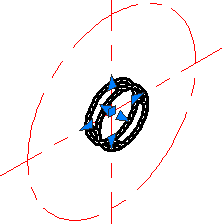
\includegraphics[scale=0.5]{duangaisolid1.png}}\hspace{30pt}
\subfloat[]{\label{fig:duangaisolid2}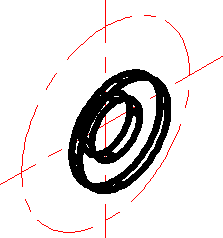
\includegraphics[scale=0.5]{duangaisolid2.png}}
\hspace{30pt}
\subfloat[]{\label{fig:duangaisolid3}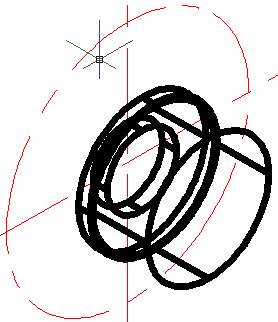
\includegraphics[scale=0.4]{duangaisolid3.png}}
\caption{端盖实体建模过程1}
\end{figure}
\begin{lstlisting}
|命令: cylinder|
|指定底面的中心点或 [三点(3P)/两点(2P)/切点、切点、半径(T)/椭|
|圆(E)]:int于|
|指定底面半径或 [直径(D)]: 12|
|指定高度或 [两点(2P)/轴端点(A)]: 5|
\end{lstlisting}
以$\phi 24$圆柱体顶圆圆心为圆心绘制$\phi 44$圆柱体,结果如图\ref{fig:duangaisolid2}所示。
\begin{lstlisting}
|命令: cylinder|
|指定底面的中心点或 [三点(3P)/两点(2P)/切点、切点、半径(T)/椭|
|圆(E)]:int于|
|指定底面半径或 [直径(D)]$<$12.0000$>$: 22|
|指定高度或 [两点(2P)/轴端点(A)]$<$5.0000$>$: 4|
\end{lstlisting}
以$\phi 44$圆柱体顶圆圆心为圆心绘制$\phi 42$圆柱体,结果如图\ref{fig:duangaisolid3}所示。。
\begin{lstlisting}
|命令: cylinder|
|指定底面的中心点或 [三点(3P)/两点(2P)/切点、切点、半径(T)/椭|
|圆(E)]:int于|
|指定底面半径或 [直径(D)]$<$22.0000$>$: 21|
|指定高度或 [两点(2P)/轴端点(A)]$<$4.0000$>$: 19|
\end{lstlisting}
以$\phi 42$圆柱体顶圆圆心为圆心绘制$\phi 62$圆柱体,结果如图\ref{fig:duangaisolid4}所示。
\begin{figure}[htbp]
\centering
\subfloat[]{\label{fig:duangaisolid4}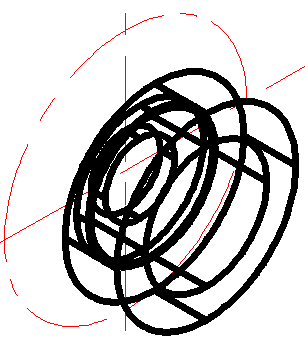
\includegraphics[scale=0.4]{duangaisolid4.png}}\hspace{30pt}
\subfloat[]{\label{fig:duangaisolid5}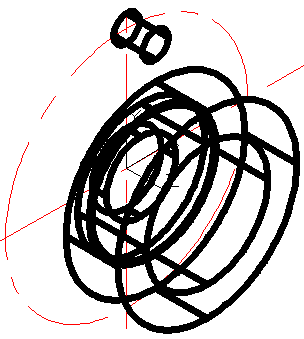
\includegraphics[scale=0.4]{duangaisolid5.png}}
\hspace{30pt}
\subfloat[]{\label{fig:duangaisolid6}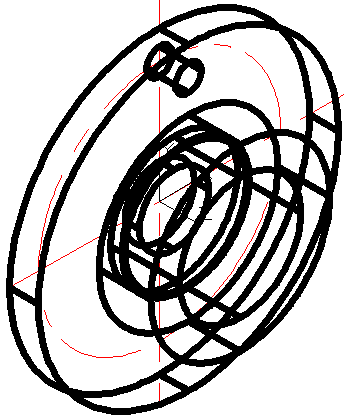
\includegraphics[scale=0.3]{duangaisolid6.png}}
\caption{端盖实体建模过程1}
\end{figure}
\begin{lstlisting}
|命令: cylinder|
|指定底面的中心点或 [三点(3P)/两点(2P)/切点、切点、半径(T)/椭|
|圆(E)]:int于|
|指定底面半径或 [直径(D)]$<$21.0000$>$: 31|
|指定高度或 [两点(2P)/轴端点(A)]$<$19.0000$>$: -18|
\end{lstlisting}
以对称中心的交点为圆心绘制$\phi 9$圆柱体,结果如图\ref{fig:duangaisolid5}所示。
\begin{lstlisting}
|命令: cylinder|
|指定底面的中心点或 [三点(3P)/两点(2P)/切点、切点、半径(T)/椭|
|圆(E)]:int于|
|指定底面半径或 [直径(D)]$<$31.0000$>$: 9|
|指定高度或 [两点(2P)/轴端点(A)]$<$-18.0000$>$:10 |
\end{lstlisting}
以对称中心的交点为圆心绘制$\phi 104$圆柱体,结果如图\ref{fig:duangaisolid6}所示。
\begin{lstlisting}
|命令: cylinder|
|指定底面的中心点或 [三点(3P)/两点(2P)/切点、切点、半径(T)/椭|
|圆(E)]:int于|
|指定底面半径或 [直径(D)]$<$31.0000$>$: 52|
|指定高度或 [两点(2P)/轴端点(A)]$<$10.0000$>$: |
\end{lstlisting}
\item 合并实体

合并实体需要用到AutoCAD中的并集命令,启动实体【并集】命令的方法有:
\begin{itemize}
\item 键盘输入UNION或UNI。
\item 点击【修改】菜单中【实体编辑】子菜单中【并集】项。
\item 点击【实体编辑】工具栏中的【并集】图标
\includegraphics[scale=0.7]{union.png}。
\end{itemize}
将$\phi 104$圆柱体和$\phi 62$圆柱体合并为一个实体。
\begin{lstlisting}
|命令:UNION|
|选择对象: 找到 1 个|
|选择对象: 找到 1 个,总计 2 个|
|选择对象:|
\end{lstlisting}
\item 三维阵列$\phi 9$圆柱体。
\begin{lstlisting}
|命令: 3darray|
|选择对象: 找到 1 个|
|选择对象:|
|输入阵列类型 [矩形(R)/环形(P)]$<$矩形$>$:p|
|输入阵列中的项目数目: 6|
|指定要填充的角度 (+=逆时针, -=顺时针)$ <360>$:|
|旋转阵列对象? [是(Y)/否(N)] $<Y>$:|
|指定阵列的中心点:|
|指定旋转轴上的第二点:|
\end{lstlisting}
\item 用差集操作完成三维建模操作。
\begin{lstlisting}
|命令: subtract |
|选择要从中减去的实体、曲面和面域...|
|选择对象: 找到 1 个|
|选择对象:  选择要减去的实体、曲面和面域...|
|选择对象: 指定对角点: 找到 9 个|
|选择对象:|
\end{lstlisting}
\item 建立三维圆角

建立三维圆角,既可使用二维【圆角】命令,也可以使用三维的【圆角边】命令。启动【圆角边】命令的方法有:
\begin{itemize}
\item 键盘输入FILLETEDGE。
\item 点击【修改】菜单中的【实体编辑】子菜单中的【圆角边】项。
\item 点击【实体编辑】工具栏中的【圆角边】图标
\includegraphics[scale=0.6]{filletedge.png}。
\end{itemize} 

\begin{lstlisting}
|命令: FILLETEDGE|
|半径 = 1.0000|
|选择边或 [链(C)/环(L)/半径(R)]:|
|选择边或 [链(C)/环(L)/半径(R)]: r|
|输入圆角半径或 [表达式(E)]$<$1.0000$>$: 3|
|选择边或 [链(C)/环(L)/半径(R)]:|  
|选择边或 [链(C)/环(L)/半径(R)]:|
|选择边或 [链(C)/环(L)/半径(R)]:|
|已选定 3 个边用于圆角。|
|按 Enter 键接受圆角或 [半径(R)]:|
\end{lstlisting}
\item 设置视觉样式为真实,其结果如图\ref{fig:duangailititu}所示。
\item 将端盖模型保存为“调压阀端盖立体图.dwg”。
\end{procedure}
%\end{procedure}
